% 这是中国科学院大学计算机科学与技术专业《计算机组成原理(研讨课)》使用的实验报告 Latex 模板
% 本模板与 2024 年 2 月 Jun-xiong Ji 完成, 更改自由 Shing-Ho Lin 和 Jun-Xiong Ji 于 2022 年 9 月共同完成的基础物理实验模板
% 如有任何问题, 请联系: jijunxoing21@mails.ucas.ac.cn
% This is the LaTeX template for report of Experiment of Computer Organization and Design courses, based on its provided Word template. 
% This template is completed on Febrary 2024, based on the joint collabration of Shing-Ho Lin and Junxiong Ji in September 2022. 
% Adding numerous pictures and equations leads to unsatisfying experience in Word. Therefore LaTeX is better. 
% Feel free to contact me via: jijunxoing21@mails.ucas.ac.cn

\documentclass[11pt]{article}

\usepackage[a4paper]{geometry}
\geometry{left=2.0cm,right=2.0cm,top=2.5cm,bottom=2.5cm}

\usepackage{ctex} % 支持中文的LaTeX宏包
\usepackage{amsmath,amsfonts,graphicx,subfigure,amssymb,bm,amsthm,mathrsfs,mathtools,breqn} % 数学公式和符号的宏包集合
\usepackage{algorithm,algorithmicx} % 算法和伪代码
\usepackage[noend]{algpseudocode} % 算法和伪代码
\usepackage{fancyhdr} % 自定义页眉页脚
\usepackage[framemethod=TikZ]{mdframed} % 创建带边框的框架
\usepackage{fontspec} % 字体设置
\usepackage{adjustbox} % 调整盒子大小
\usepackage{fontsize} % 设置字体大小
\usepackage{tikz,xcolor} % 绘制图形和使用颜色
\usepackage{multicol} % 多栏排版
\usepackage{multirow} % 表格中合并单元格
\usepackage{pdfpages} % 插入PDF文件
\usepackage{listings} % 在文档中插入源代码
\usepackage{wrapfig} % 文字绕排图片
\usepackage{bigstrut,multirow,rotating} % 支持在表格中使用特殊命令
\usepackage{booktabs} % 创建美观的表格
\usepackage{circuitikz} % 绘制电路图
\usepackage{zhnumber} % 中文序号(用于标题)
\usepackage{tabularx} % 表格折行

\definecolor{dkgreen}{rgb}{0,0.6,0}
\definecolor{gray}{rgb}{0.5,0.5,0.5}
\definecolor{mauve}{rgb}{0.58,0,0.82}
% \lstset{
%   frame=tb,
%   aboveskip=3mm,
%   belowskip=3mm,
%   showstringspaces=false,
%   columns=flexible,
%   framerule=1pt,
%   rulecolor=\color{gray!35},
%   backgroundcolor=\color{gray!5},
%   basicstyle={\small\ttfamily},
%   numbers=none,
%   numberstyle=\tiny\color{gray},
%   keywordstyle=\color{blue},
%   commentstyle=\color{dkgreen},
%   stringstyle=\color{mauve},
%   breaklines=true,
%   breakatwhitespace=true,
%   tabsize=3,
% }



\lstset{
    % basicstyle=\ttfamily\small,
    basicstyle=\ttfamily\footnotesize,
    keywordstyle=\color{blue},
    commentstyle=\color{gray},
    numbers=left,
    numberstyle=\tiny,
    breaklines=true,
    frame=single,
}

\lstdefinelanguage{Verilog}{
    morekeywords={always, and, assign, attribute, begin, buf, bufif0, bufif1, case, casex, casez, 
                 cmos, deassign, default, defparam, disable, edge, else, end, endattribute, 
                 endcase, endfunction, endmodule, endprimitive, endspecify, endtable, endtask, 
                 event, for, force, forever, fork, function, highz0, highz1, if, ifnone, initial, 
                 inout, input, integer, join, large, macromodule, medium, module, nand, negedge, 
                 nmos, nor, not, notif0, notif1, or, output, parameter, pmos, posedge, primitive, 
                 pull0, pull1, pulldown, pullup, rcmos, real, realtime, reg, release, repeat, 
                 rnmos, rpmos, rtran, rtranif0, rtranif1, scalared, signed, small, specify, 
                 specparam, strong0, strong1, supply0, supply1, table, task, time, tran, tranif0, 
                 tranif1, tri, tri0, tri1, triand, trior, trireg, unsigned, vectored, wait, wand, 
                 weak0, weak1, while, wire, wor, xnor, xor},
    morekeywords=[2]{`define, `undef, `ifdef, `ifndef, `else, `elsif, `endif, `include, 
                    `resetall, `timescale, `celldefine, `endcelldefine, `default_nettype, 
                    `unconnected_drive, `nounconnected_drive},
    morekeywords=[3]{\$display, \$write, \$strobe, \$monitor, \$time, \$stime, \$realtime, 
                    \$finish, \$stop, \$dumpfile, \$dumpvars, \$dumpon, \$dumpoff, \$dumpall, 
                    \$dumpflush, \$dumplimit, \$random, \$readmemb, \$readmemh},
    morecomment=[l]{//},
    morecomment=[s]{/*}{*/},
    morestring=[b]",
    sensitive=true,
    keywordstyle=\color{blue}\bfseries,
    keywordstyle=[2]\color{purple}\bfseries,
    keywordstyle=[3]\color{orange}\bfseries,
    stringstyle=\color{red},
    numberstyle=\tiny\color{gray},
    stepnumber=1,
    numbersep=10pt,
    backgroundcolor=\color{white},
    showspaces=false,
    showstringspaces=false,
    showtabs=false,
    frame=single,
    tabsize=4,
    captionpos=b,
    breaklines=true,
    breakatwhitespace=false,
    title=\lstname,
    escapeinside={\%*}{*},
    morekeywords={*,...}
}









% 轻松引用, 可以用\cref{}指令直接引用, 自动加前缀. 
% 例: 图片label为fig:1
% \cref{fig:1} => Figure.1
% \ref{fig:1}  => 1
\usepackage[capitalize]{cleveref}
% \crefname{section}{Sec.}{Secs.}
\Crefname{section}{Section}{Sections}
\Crefname{table}{Table}{Tables}
\crefname{table}{Table.}{Tabs.}

% \setmainfont{Palatino Linotype.ttf}
% \setCJKmainfont{SimHei.ttf}
% \setCJKsansfont{Songti.ttf}
% \setCJKmonofont{SimSun.ttf}
\punctstyle{kaiming}
% 偏好的几个字体, 可以根据需要自行加入字体ttf文件并调用

\renewcommand{\emph}[1]{\begin{kaishu}#1\end{kaishu}}

% 对 section 等环境的序号使用中文
% \renewcommand \thesection{\zhnum{section}、}
% \renewcommand \thesubsection{\arabic{section}}


%%%%%%%%%%%%%%%%%%%%%%%%%%%
%改这里可以修改实验报告表头的信息
\newcommand{\name}{裴晨皓\ 竹彦博\ 纪弘璐}
\newcommand{\studentNum}{2023K8009916003\ \ \ \ 2023K8009916001\ \ \ \ 2023K8009916002}
\newcommand{\major}{计算机科学与技术}
\newcommand{\labNum}{Project 3}
\newcommand{\labName}{添加用户态指令设计专题实验}
%%%%%%%%%%%%%%%%%%%%%%%%%%%

\begin{document}

\begin{center}
  \LARGE \bf 中国科学院大学 \\《计算机体系结构(研讨课)》实验报告
\end{center}

\begin{center}
  \emph{姓名} \underline{\makebox[11em][c]{\name}} 
  % 如果名字比较长, 可以修改box的长度"8em"为其他值
  \emph{学号} \underline{\makebox[30.5em][c]{\studentNum}}\\
  \emph{专业} \underline{\makebox[12em][c]{\major}}
  \emph{实验项目编号} \underline{\makebox[5em][c]{\labNum}}
  \emph{实验名称} \underline{\makebox[16em][c]{\labName}}\\
\end{center}

% \begin{center}
%   \begin{tabularx}{\textwidth}{|lX|}
%     \hline
%     注1: & 撰写此 Word 格式实验报告后以 PDF 格式保存 SERVE CloudIDE 的 \texttt{/home/serve-ide/ cod-lab/reports} 目录下(注意:reports 全部小写)。文件命名规则:\texttt{prjN.pdf},其中 \texttt{prj} 和后缀名 \texttt{pdf} 为小写,\texttt{N} 为1至4的阿拉伯数字。例如:\texttt{prj1.pdf}。PDF 文件大小应控制在 5MB 以内。此外,实验项目5包含多个选做内容,每个选做实验应提交各自的实验报告文件,文件命名规则:\texttt{prj5-projectname.pdf},其中``-''为英文标点符号的短横线。文件命名举例:\texttt{prj5-dma.pdf}。具体要求详见实验项目5讲义。 \\

%     注2: & 使用\texttt{git add}及\texttt{git commit}命令将实验报告\texttt{PDF}文件添加到本地仓库master分支,并通过\texttt{git push}推送到实验课SERVE GitLab远程仓库master分支(具体命令详见实验报告)。 \\

%     注3: & 实验报告模板下列条目仅供参考,可包含但不限定如下内容。实验报告中无需重复描述讲义中的实验流程。\\
%     \hline
%   \end{tabularx}
% \end{center}

  

\section{实验简介}
本次实验的内容主要是在原有的流水线CPU中进一步添加算术逻辑运算、乘除法运算、转移和访存这四类用户态指令。在此基础上,本组同学又额外自行完成了除法器模块和两级流水乘法器的设计,并通过了测试。

\section{设计方案介绍}
\subsection{总体思路}
借助已有的CPU设计,本组同学结合教材讲解与指令集手册内容,把指令的添加分为控制通路、数据通路和功能实现三个部分,充分利用“复用”思想,遵循原有的设计逻辑,向CPU中添加新的指令支持。下面将按照设计时分成的三个部分进行介绍。

特别地,由于引入新的模块(乘/除法器),乘除法的功能实现将单独介绍。

下图为经过本次实验修改后的处理器结构框图:
\begin{lstlisting}
\
\
\
\
\       
\
\
\                皇帝的新图
\
\
\
\
\
\
\
\end{lstlisting}
\subsection{控制通路(整体)}

\subsubsection{指令译码与各模块操作码生成(ID)}

延续原有的设计思路,结合指令的操作码,利用译码器对每一条新添加的指令单独译码,生成专门的控制信号inst_xxx(例如inst_div_wu、inst_mod_w等)。

新增加的指令涉及的部分运算需求,可以充分利用原有alu的功能,在生成alu_op时采用“或”逻辑,把新增指令的inst_xxx信号加入其中。比如新增的ld_b计算访存地址时要使用加法,可以用此法使之与原有的add_w指令共享alu的加法功能。

由于引入的乘除法和访存指令各自都有多条,所以采用mul_op、div_op和mem_op的方式进行区分,与alu_op类似,采用独热码的方式。以mul_op为例:
\begin{lstlisting}[language=Verilog, caption={mul_op(独热码)}]
assign mul_op = {inst_mulh_wu, inst_mulh_w, inst_mul_w};
\end{lstlisting}


\subsubsection{数据选择(主要在ID)}

新增的指令很多都涉及读寄存器操作,所以要把新增指令中以rd为目标读寄存器号者的inst_xxx信号通过“或”运算加入src_reg_is_rd信号(如bge、bgeu等),复用src_reg_is_rd控制寄存器堆2号读端口地址是rd还是rk。
\begin{lstlisting}[language=Verilog, caption={src\_reg\_is\_rd信号}]
assign src_reg_is_rd = inst_beq | inst_bne | inst_blt | inst_bge | inst_bltu | inst_bgeu | inst_st_b | inst_st_h | inst_st_w;
\end{lstlisting}

同理,用这种“附加并复用”的方法处理alu输入操作数的选择信号src1_is_pc、src2_is_imm,还以此法修改了标记访存指令、在判断写后读冲突的同时选择前递数据的res_from_mem信号。此外,仿照res_from_mem,我们又引入了res_from_div和res_from_mem,用于在EX和MEM阶段生成握手信号。

(判定寄存器写操作指令的gr_we、判定store指令的mem_we等信号的修改方式也类似,后文不再赘述。)

\subsubsection{“写后读”冲突处理与旁路设计的修改(ID)}

根据课上老师的提示,我们自己设计的乘法器在性能方面会劣于调用Xilinx\ IP实现出的乘法部件——关键路径会长一些。如果再加上前递通路传回ID参与其他逻辑(比如分支指令条件判断),就会进一步增大关键路径,严重影响性能。因此,为了尽可能减少隐患,我们决定不对乘法结果采用前递技术——引入控制信号mul_div_hazzard:

\begin{lstlisting}[language=Verilog, caption={caption text}]
assign mul_div_hazzard = in_valid & (
    rf_raddr1 == dest_out && !src1_is_pc && gr_we_out && (res_from_mul_out || res_from_div_out) && out_valid ||
    rf_raddr2 == dest_out && !src2_is_imm && gr_we_out && (res_from_mul_out || res_from_div_out) && out_valid ||
    rf_raddr1 == MEM_dest && !src1_is_pc && MEM_gr_we && (MEM_res_from_mul || MEM_res_from_div) && MEM_valid ||
    rf_raddr2 == MEM_dest && !src2_is_imm && MEM_gr_we && (MEM_res_from_mul || MEM_res_from_div) && MEM_valid ||
    rf_raddr1 == WB_dest && !src1_is_pc && WB_gr_we && (WB_res_from_mul || WB_res_from_div) && WB_valid ||
    rf_raddr2 == WB_dest && !src2_is_imm && WB_gr_we && (WB_res_from_mul || WB_res_from_div) && WB_valid
);
\end{lstlisting}

这一设计在实现思路上仿照了写后读的判断逻辑,又另外加入了“与ID冲突的阶段内部是一条乘法或除法指令”的条件。使用这一信号即可准确判定是否有乘法指令与当前ID的指令发生写后读冲突。


\subsubsection{对流水线控制信号的修改(ID、EX、MEM)}

按照原有设计逻辑,每个阶段的ready_go信号意味着一种能力的具备,有“can”之含义(而非will),表示该阶段工作完成,准备好进入下一个阶段(但不一定真的马上(will)进入下一阶段。特别地,如果当前阶段无效,那么ready_go也为1——我们认为无效的“空穴”持续具备移动的能力)。

\begin{enumerate}
    \item 由于ID阶段屏蔽掉乘法指令的前递,所以在ready_go判断中引入了mul_div_hazzard信号。如果mul_div_hazzard满足,就要一直阻塞ID至前面冲突的指令做完WB阶段.
    \item EX和MEM涉及与乘/除法器子系统的握手。除了阶段无效可以ready_go外,在阶段有效时,只有“既不是没有req/resp成功的乘法指令,并且也不是没有req/resp成功的除法指令”条件满足,才可以ready_go。
\end{enumerate}
具体实现如下:

\begin{lstlisting}[language=Verilog, caption={修改后的ready_go}]
// ID:
assign ready_go = ~in_valid | ~load_use_sign & ~mul_div_hazzard;
// EX:
assign ready_go = !in_valid ||
					  !(res_from_mul && !(from_mul_req_ready && to_mul_req_valid)) &&
					  !(res_from_div && !(from_div_req_ready && to_div_req_valid));
// MEM:
assign ready_go = !in_valid ||
                      !(res_from_mul && !(to_mul_resp_ready && from_mul_resp_valid)) &&
                      !(res_from_div && !(to_div_resp_ready && from_div_resp_valid));
\end{lstlisting}




\subsection{数据通路(整体)}

\subsubsection{“result”的收集}
原先,在EX得到alu的运算结果,WB得到load的结果,要在WB使用选择器根据指令类型选出写回寄存器的结果。现在增加乘除法器模块后,会在MEM阶段收集到乘/除法结果,所以在MEM阶段要额外加入对alu、乘法器、除法器(商和余数)的结果选择,然后传递到WB阶段继续进行选择。

\subsubsection{流水寄存器的数据传递(这时“控制信号”也可视为被传递的数据)}
在ID阶段增加的许多信号要在后续阶段使用,于是要通过流水寄存器逐级传递下去,本次新增的mul_op、div_op等信号要传到计算乘除法的EX和MEM,mem_op要传到MEM和WB用于发送访存请求和接收load结果。


\subsection{功能实现(局部)}

\subsubsection{算术逻辑运算指令}
新增的移位、逻辑运算、算术运算都能够复用alu的功能,利用原有算术逻辑运算指令的数据和控制通路进行运算。特别地,新增的andi、ori和xori指令用到了零扩展i12的立即数,只要新增控制信号need_ui12,对imm的生成稍作修改即可。

\subsubsection{访存指令}

在MEM阶段,由于引入了半字和字节访存,所以目标地址可能不是4字节对齐的,要把最低两位清0,得到实际访存地址:
\begin{lstlisting}[language=Verilog, caption={访存地址}]
assign data_sram_addr  = result & ~32'b11;
\end{lstlisting}

如果是非“全字”的store指令,根据操作的字节数(mem_op)和目标地址相对实际访问的起始地址的偏移量(目标地址result的末两位)形成字节掩码(字节写使能位),发送给数据内存:
\begin{lstlisting}[language=Verilog, caption={store字节写使能}]
assign data_sram_we = {4{mem_we && valid && in_valid}} & (
                        ({4{mem_op[5]}} & (4'b0001 << result[1: 0])) |  // SB
                        ({4{mem_op[6]}} & (4'b0011 << result[1: 0])) |  // SH
                        ({4{mem_op[7]}} & 4'b1111)  // SW;
                    );
\end{lstlisting}
有了写使能的限制,就可以采取教材中提到的较好的发送store数据的方法——将Byte重复4次,将Half\ Word重复2次,无论地址的相对偏移如何,结合写使能,选到的字节/半字总是从寄存器读出的最低字节/半字:

\begin{lstlisting}[language=Verilog, caption={store数据}]
assign data_sram_wdata = {32{mem_op[5]}} & {4{rkd_value[7:0]}} | 
                             {32{mem_op[6]}} & {2{rkd_value[15: 0]}} |
                             {32{mem_op[7]}} & rkd_value;
\end{lstlisting}

如果是非“全字”的load指令,依旧先根据mem_op对数据的字节数(Byte/Half\ Word)分类,再借助地址偏移(result的末两位)形成多路选择器,在从内存得到的4字节数据中选出需要的部分,进行位扩展后形成“mem_result”:

\begin{lstlisting}[language=Verilog, caption={load数据}]
assign mem_result   = 
        {32{mem_op[0] | mem_op[3]}} &   // LB & LBU
            ({32{result[1: 0] == 2'b00}} & {{24{mem_op[0] & data_sram_rdata[7]}}, data_sram_rdata[7: 0]} | 
    		{32{result[1: 0] == 2'b01}} & {{24{mem_op[0] & data_sram_rdata[15]}}, data_sram_rdata[15: 8]} | 
			{32{result[1: 0] == 2'b10}} & {{24{mem_op[0] & data_sram_rdata[23]}}, data_sram_rdata[23: 16]} | 
			{32{result[1: 0] == 2'b11}} & {{24{mem_op[0] & data_sram_rdata[31]}}, data_sram_rdata[31: 24]}) |
		{32{mem_op[1] | mem_op[4]}} &   // LH & LHU
			({32{result[1: 0] == 2'b00}} & {{16{mem_op[1] & data_sram_rdata[15]}}, data_sram_rdata[15: 0]} |
			{32{result[1: 0] == 2'b10}} & {{16{mem_op[1] & data_sram_rdata[31]}}, data_sram_rdata[31: 16]}) |
	 	{32{mem_op[2]}} & data_sram_rdata;  // LW
\end{lstlisting}

位扩展的方法比较巧妙,以LH/LHU的情况为例:将mem_op[1]和load出的半字数据“与”在一起,然后扩展。mem_op[1]代表LH,是有符号的,“与”运算结束后得到的就是数据的符号位;若是无符号的LHU,则mem_op[1]为0,“与”之后必为0,位扩展时也自然全用0填充。

\subsubsection{转移指令}
新增的转移指令条件判断需要比较两个寄存器值的大小关系,而非仅仅判断是否相等。我们仿照rj_eq_rd信号,引入了另外两个用于无符号数和有符号数比大小的信号:

\begin{lstlisting}[language=Verilog, caption={转移指令条件判断信号}]
assign rj_lt_rd = ($signed(rj_value) < $signed(rkd_value));
assign rj_ltu_rd = (rj_value < rkd_value);
\end{lstlisting}

然后根据具体指令的inst_xxx和条件判断结果,复用判断转移与否的br_taken和br_target信号即可。

\subsubsection{乘除法指令}
\noindent
与乘除法器“子系统”的交互——握手(EX、MEM):

做乘除法指令时,CPU利用两个流水级进行运算,在EX级向相应运算模块发送数据,在MEM级接收结果。如果把乘/除法器视为正常的(例如物理内存等)子系统,那么它们与CPU进行交互时就需要用到握手信号。

在EX阶段,以除法指令为例,CPU使用req_valid发送运算请求,申请向除法器发送数据:

\begin{lstlisting}[language=Verilog, caption={CPU的除法运算请求}]
assign to_div_req_valid = in_valid && res_from_div;
\end{lstlisting}
只要EX有效(in_valid)且内部是除法指令(res_from_mul/div),就应当发请求。

进而,在MEM阶段,CPU使用resp_ready向除法器表明自己准备好接收结果:
\begin{lstlisting}[language=Verilog, caption={CPU的除法运算接收准备}]
assign to_div_resp_ready = in_valid && res_from_div;
\end{lstlisting}
同理,如果MEM有效且在做除法指令,就能够接收结果。


乘/除法器的具体设计见后文对的阐释。




\subsection{乘法器}

按照教材上提到的采用3:2压缩的华莱士树,我们按照给出的电路图进行连线先实现了组合逻辑乘法器模块(module\  multiplier),然后在汪老师的建议下从华莱士树的第2、3层之间切分为了二级流水乘法器。

\subsubsection{乘法器接口}

模块接口的定义如下:

\begin{table}[H]
    \centering
    \begin{tabular}{cccc}\hline
        名称                & 方向与类型 & 位宽 & 含义                                    \\ \hline
        mul_clk             & in(wire)   & 1    & 时钟信号                                \\
        reset               & in(wire)   & 1    & 复位信号                                \\ \hline
        mul_op              & in(wire)   & 3    & 操作码                                  \\
        x                   & in(wire)   & 32   & 乘数1                                   \\
        y                   & in(wire)   & 32   & 乘数2                                   \\\hline
        to_mul_req_valid    & in(wire)   & 1    & 握手信号,表明输入有效                  \\
        from_mul_req_ready  & out(wire)  & 1    & 握手信号,表明准备好接收输入            \\
        to_mul_resp_ready   & in(wire)   & 1    & 握手信号,表明外界准备好接收乘法器的输出\\
        from_mul_resp_valid & out(wire)  & 1    & 握手信号,表明运算完成,输出有效        \\ \hline
        result              & out(wire)  & 64   & 积                                      \\ \hline
    \end{tabular}
\end{table}

\subsubsection{组合逻辑乘法器结构框图及实现原理}

按照教材的说明,我们实现了一个既可以做有符号乘法运算,又可以做无符号乘法运算的33位有符号乘法器。

此处引用书上的内容:下面是乘法器以及其核心部件“华莱士树”的结构框图:

\begin{figure}[H]
  \centering
  \subfigure[17个部分积相加的1位华莱士树(左侧“C5\textasciitilde 9”应为“C5\textasciitilde 8”)]{
    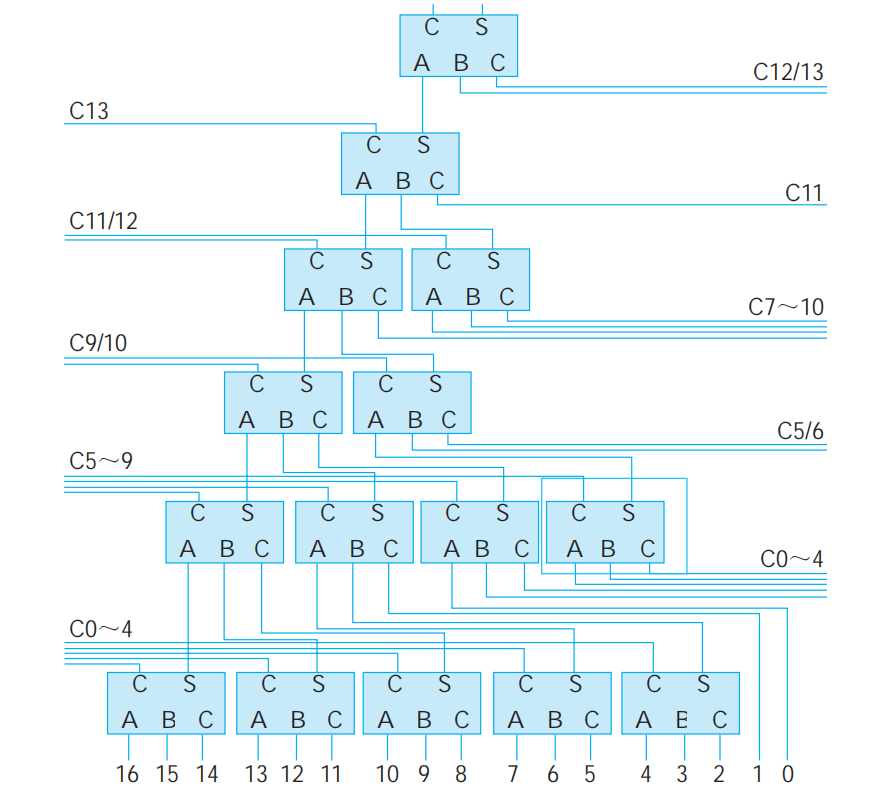
\includegraphics[width=0.41\textwidth]{fig/17个部分积相加的1位华莱士树.png}
  }
  \subfigure[33位定点补码乘法器结构]{
    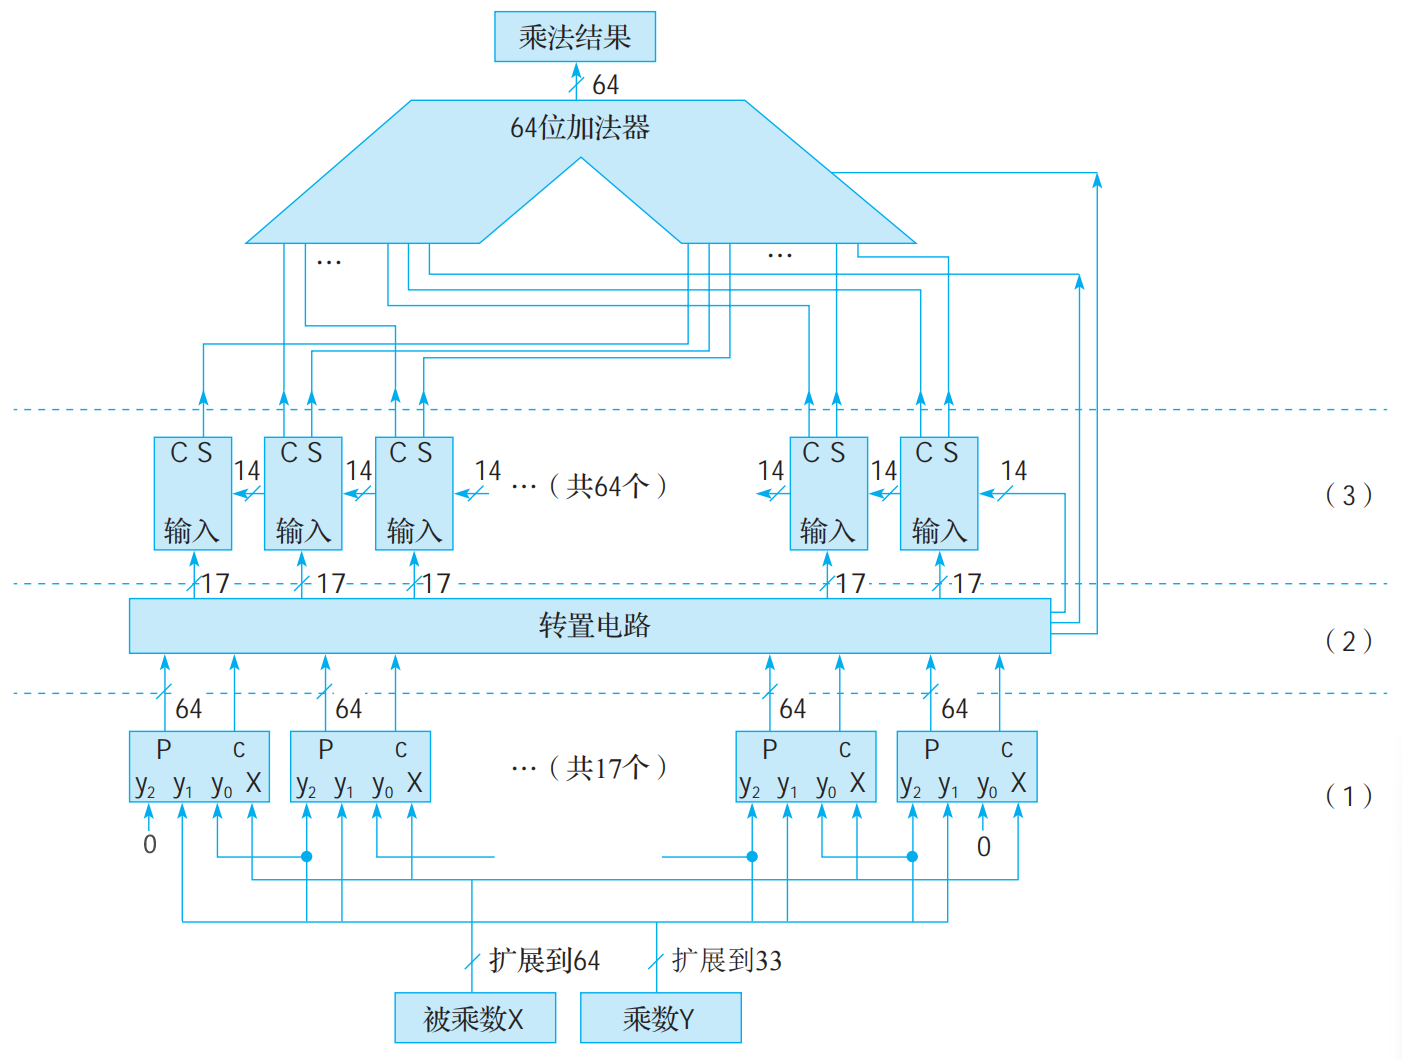
\includegraphics[width=0.55\textwidth]{fig/33.png}
  }
  \caption{“华莱士树”与“乘法器总体结构”框图}
\end{figure}

注:教材未给出优化后的33位定点补码乘法器结构图,此处的结构图(b)由教材的32位版本修改而来。

实现上,在除法器模块multiplier内部,我们分别设计了wallace(1位华莱士树)模块、booth(两位booth乘法部分积生成)模块以及起运算辅助作用的full_adder(1位全加器)辅助模块。基本完全按照框图所示的电路图进行连线,故此处不额外展示代码。

如上图中的图(b)所示,第(1)部分实例化了17个booth模块,运算得到17个64位的部分积,送给第(2)部分的转置电路(在顶层模块multiplier内部直接实现),转化成64组(部分积做加法时)每一位上的17个加数,送给第(3)部分。第(3)部分实例化64个wallace,wallace内部利用“保留进位加法”原理进行3:2压缩,通过6层压缩,将17个加数变成2个(最终的和S与进位C),而中间产生的14进位信号C0 \textasciitilde C13则传递给对更高1位进行计算的wallace。

最后用一个64位加法器将每一位的值S与来自低位的进位C相加,得到最终的乘积result。

\subsubsection{流水化改进}

在华莱士树内部进行流水化拆分时,每一层产生的S信号直接向更高层传递即可,跨流水级处使用流水寄存器进行过渡,逻辑十分简单。而每一棵华莱士树运算过程中产生的进位信号C0 \textasciitilde C13,需要传给下一棵树,这就涉及到不同华莱士树模块之间的数据通路设计,应当特别注意。为了使情况更加直观,下面给出相邻华莱士树数据通路示意图:

\begin{figure}[H]
    \centering
    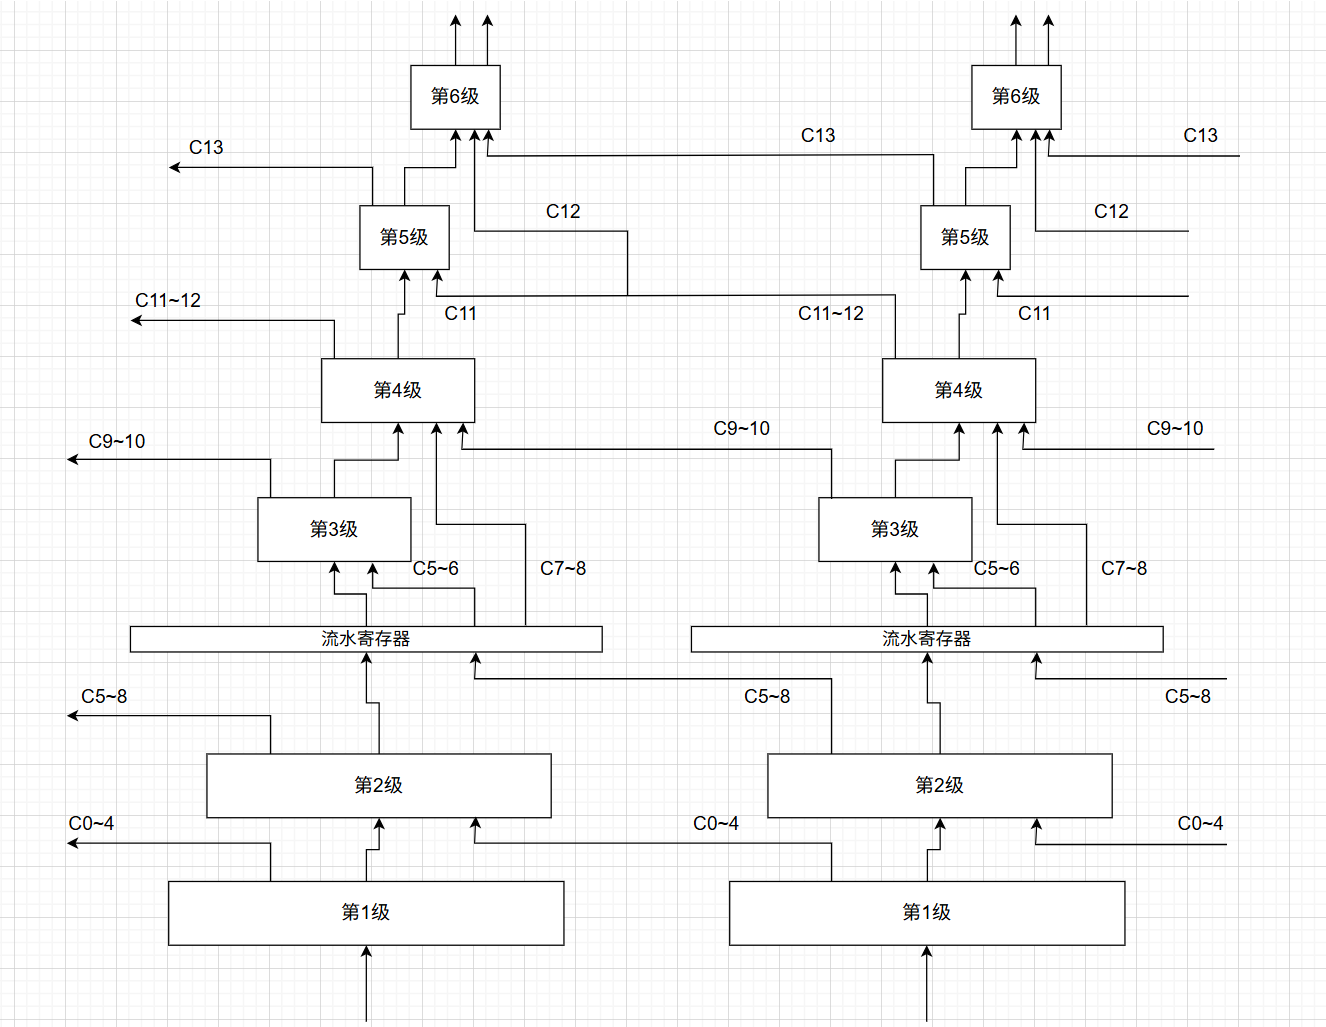
\includegraphics[width=0.8\textwidth]{fig/华莱士流水示意图.png}
    \caption{相邻两棵华莱士树的数据通路(流水化)}
\end{figure}

切分流水时,我们不能以“棵”为单位看待华莱士树,而是应该以另一种视角,将这64棵树视作“森林”,考虑森林上下两个部分(第1、2层和第3、4、5、6层)之间的数据通路:在这两个部分之间插入流水寄存器,所有下半部分输出的数据都应当先存入流水寄存器,然后才能给上半部分使用。结合上面流水化后的数据通路示意图,代码自然不难写出。

结合乘法器“当前周期输入,下一周期输出”的特点,设计如下的乘法器控制信号(带有req和resp的为握手信号):

\begin{lstlisting}[language=Verilog, caption={乘法器控制信号}]
    assign do_mul = to_mul_req_valid && from_mul_req_ready;
    always @(posedge mul_clk) begin
        if(reset) begin
            from_mul_resp_valid_reg <= 1'b0;
        end
        else if(do_mul) begin
            from_mul_resp_valid_reg <= 1'b1;
        end
    end
    assign from_mul_resp_valid = from_mul_resp_valid_reg;
    assign from_mul_req_ready = to_mul_resp_ready;
\end{lstlisting}

\begin{enumerate}
    \item 如果输入握手成功(req),则do_mul为1,允许乘法器流水线流动(进行运算),接受当前新的输入,在第二级算出新的结果。
    \item 进行了乘法运算(do_mul),那么输出结果(resp)就一定会变为有效(valid)。
    \item 如果外界能够接受(resp_ready)乘法器第二级的输出结果,那么乘法器也就做好了接收新输入的准备(req_ready)。
\end{enumerate}

下面是流水寄存器的设计:S2_reg接收第1级流水的最终输出S2;Cin_reg保存前一棵树送来的进位信号Cin:

\begin{lstlisting}[language=Verilog, caption={华莱士树流水寄存器}]
    // register for pipeline
    reg [13:0] Cin_reg;
    reg [ 3:0] S2_reg;
    always @(posedge mul_clk) begin
        if(reset) begin
            Cin_reg <= 14'd0;
            S2_reg <= 4'd0;
        end 
        else if(do_mul)begin
            Cin_reg <= Cin;
            S2_reg <= S2;
        end
    end
\end{lstlisting}

然后结合图3按需连线,形成第二级流水中华莱士树每一层的输入——以第4层为例:

\begin{lstlisting}[language=Verilog, caption={华莱士树第4层的输入}]
assign in4 = {S3, Cin[10:9], Cin_reg[8:7]};
\end{lstlisting}

需要特别注意:第二级流水内,并非所有的进位输入都来自流水寄存器,有些进位信号是跨越流水级传递的(C7、C8),还有一些只在同一流水级内传递(C9、C10)——同级内部自然也没有流水寄存器可言。。


\subsection{除法器}
除法器作为单独的一个模块(module\  Div),由本组同学尝试使用chisel进行实现,转化成Verilog后接入到流水线CPU中。

按照教材的指导,采用的运算方法为:做无符号数除法时,采用恢复余数法;如果是有符号数除法,则先用两个输入操作数的绝对值进行无符号数除法,然后根据被除数和除数的符号确定商和余数的符号。

\subsubsection{除法器接口}

模块接口定义如下:

\begin{table}[H]
    \centering
    \begin{tabular}{cccc}\hline
        名称                  & 方向与类型 & 位宽 & 含义                                    \\ \hline
        clock                 & in(wire)   & 1    & 时钟信号                                \\
        reset                 & in(wire)   & 1    & 复位信号                                \\ \hline
        io_in_valid           & in(wire)   & 1    & 握手信号,表明输入有效                  \\
        io_in_ready           & out(wire)  & 1    & 握手信号,表明准备好接收输入            \\
        io_out_ready          & in(wire)   & 1    & 握手信号,表明外界准备好接收除法器的输出\\
        io_out_valid          & out(wire)  & 1    & 握手信号,表明运算完成,输出有效        \\ \hline
        io_in_bits_divOp      & in(wire)   & 4    & 操作码                            \\
        io_in_bits_dividend   & in(wire)   & 32   & 被除数                                  \\
        io_in_bits_divisor    & in(wire)   & 32   & 除数                                    \\
        io_out_bits_quotient  & out(wire)  & 32   & 商                                      \\
        io_out_bits_remainder & out(wire)  & 32   & 余数                                    \\ \hline
    \end{tabular}
    \caption{除法器模块接口}
\end{table}

其中,握手信号作为控制信号,在握手成功(in(或者out)的valid和ready同时拉高)时,数据通路对数据进行传递,in握手成功则数据进入乘法器,out握手成功则从乘法器输出计算结果。

\subsubsection{除法器结构框图}
下图为除法器结构框图:
\begin{figure}[H]
    \centering
    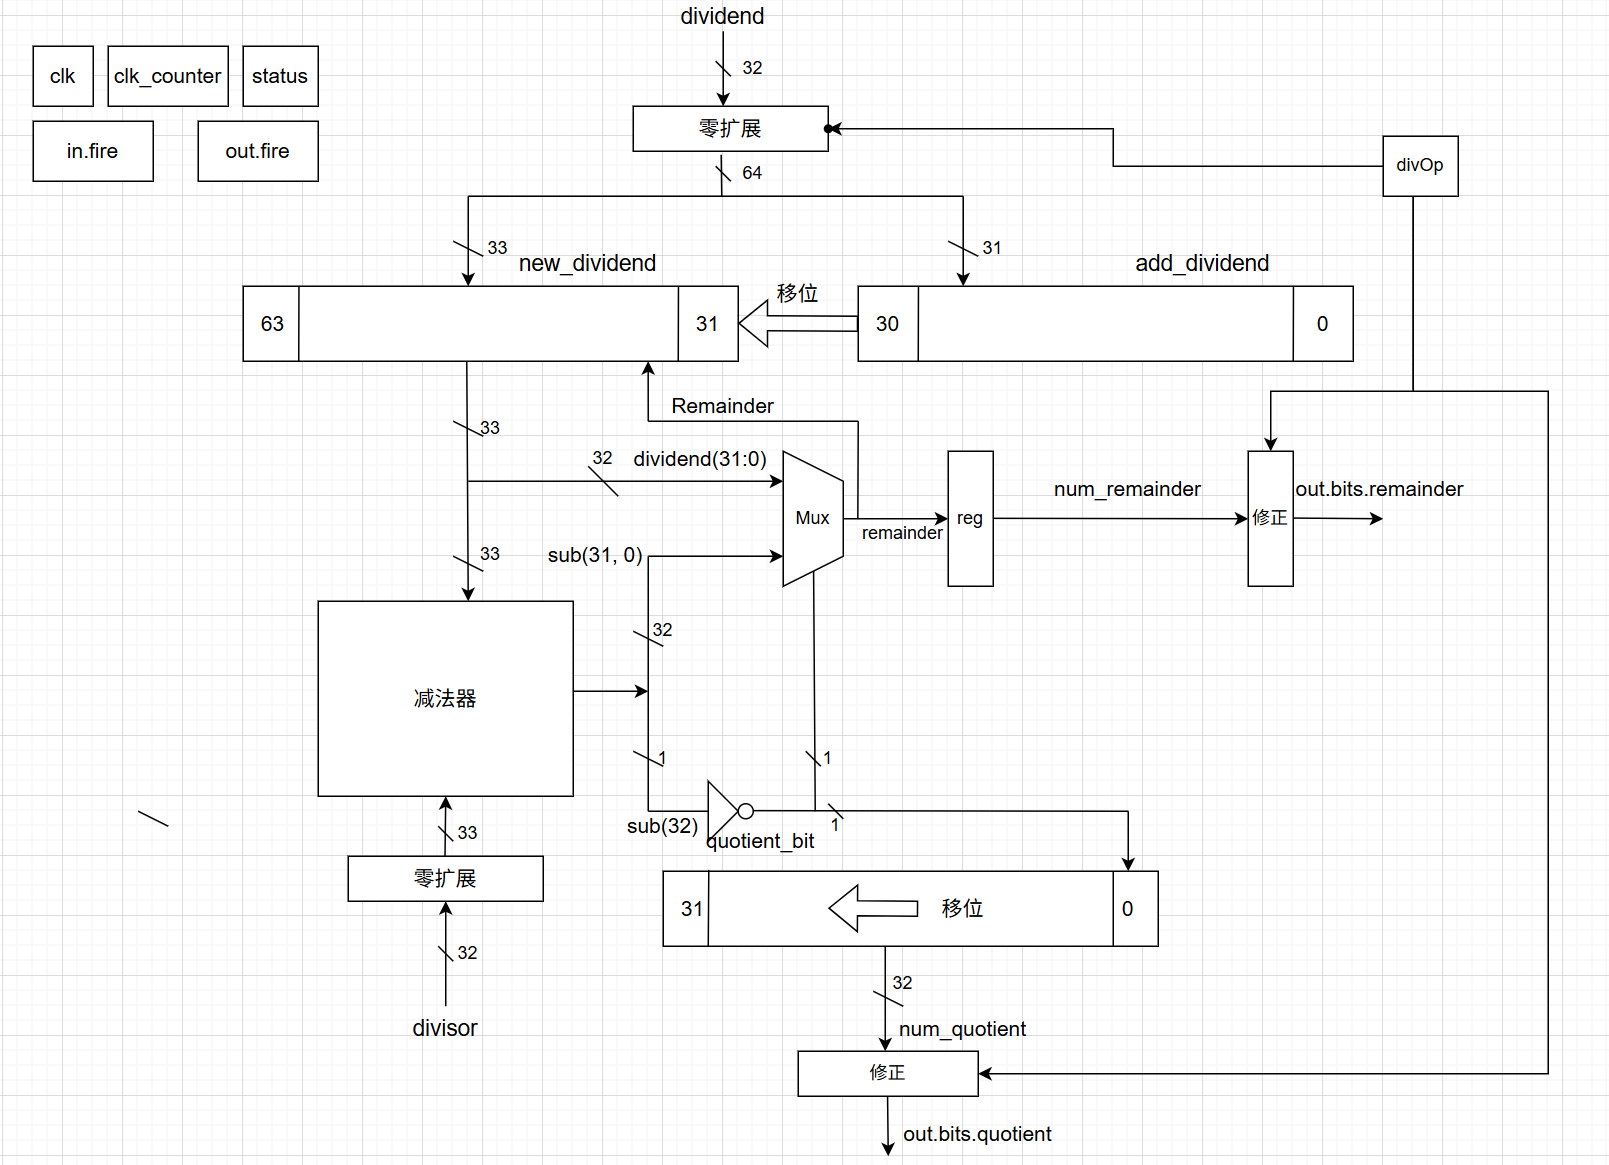
\includegraphics[width=0.8\textwidth]{fig/取法器.png}
    \caption{除法器结构框图}
\end{figure}


\subsubsection{除法器设计思路}

我们引入了Chisel3基本构件,借助Decoupled(握手)、Cat(按位拼接)、Fill(重复位填充)工具进行设计。此外,定义了BitUtils、Status、DivOp这三个对象作为辅助,分别用于操作数调整、状态定义和操作码定义。BitUtils中,实现了用于对操作数进行0扩展的zext函数,以及取绝对值的abs函数。Status对象内定义的两个状态用于区分除法器空闲(IDLE)还是正在工作(BUSY);DivOp对象内用独热码区分了四种除法操作DIV(div.w)、DIVU(div.wu)、REM(mod.w)、REMU(mod.wu)。这部分代码逻辑较为直白,此处不浪费篇幅。



在除法器模块内部,把divOp(操作码)、dividend(被除数)和divisor(除数)三者打包进DivReq,作为“输入数据包(in)”;把quotient(商)和remainder(余数)打包进DivResp,作为“输出数据包(out)”。借助Flipped和Decoupled工具,使输入输出附带握手信号,io.in.fire代表输入握手成功,io.out.fire代表输出握手成功。
\begin{lstlisting}[caption={IO接口}]
val io = IO(new Bundle {
        val in = Flipped(Decoupled(new DivReq()))
        val out = Decoupled(new DivResp())
    })
\end{lstlisting}

除法器发给外界的握手信号为io.in.ready和io.out.valid——当除法器在IDLE空闲状态时,显然应该准备好接收输入;当除法器工作(BUSY)到完成全部计算时(clk_counter用于记录迭代运算周期数,到32拍时完成),输出结果有效:

\begin{lstlisting}[caption={除法器发向外部的握手信号}]
io.in.ready := status === Status.IDLE
io.out.valid := (clk_counter === 32.U) && (status === Status.BUSY) 
\end{lstlisting}


试减操作是恢复余数除法的核心内容,专门定义一个组合逻辑模块来完成:
\begin{lstlisting}[caption={试减模块(div_iter)}]
def div_iter(dividend: UInt, divisor: UInt): (Bool, UInt) = {
        val sub = Wire(UInt(33.W))
        sub := dividend - divisor
        val quotient_bit = (sub(32) === 0.B)
        val remainder = Wire(UInt(32.W))
        remainder := Mux(quotient_bit, sub(31, 0), dividend(31, 0))
        (quotient_bit, remainder)
}
\end{lstlisting}
这一模块把64位被除数中参与相减的33位与33位的除数相减,得到结果sub,根据sub的符号位确定当前上商的一位商值quotient_bit(sub为正则够减,上商1;反之上商0),然后根据quotient_bit确定当前步骤的余数remainder,利用Mux选择减法结果sub或是还原成原来的dividend(恢复余数)。

完整运算的过程则通过when-elsewhen的组合,用时序逻辑实现(类似状态机,不被阻塞的情况下共34拍):
\begin{enumerate}
    \item 数据输入:
    \begin{lstlisting}[caption={数据输入}]
    val status = RegInit(Status.IDLE)
    when (io.in.fire) {
        status := Status.BUSY
        dividend := io.in.bits.dividend
        divisor := io.in.bits.divisor
        divOp := io.in.bits.divOp
        clk_counter := 0.U
        val zext_in_dividend = Wire(UInt(64.W))
        zext_in_dividend := BitUtils.zext(Mux(io.in.bits.divOp === DivOp.DIV || io.in.bits.divOp === DivOp.REM, BitUtils.abs(io.in.bits.dividend), io.in.bits.dividend), 32, 64)
        new_dividend := zext_in_dividend(63, 31)
        add_dividend := zext_in_dividend(30, 0)
    }
    \end{lstlisting}

    初始时,状态机处于空闲的IDLE状态。当输入握手成功时,进入BUSY工作状态,将输入的操作数和divOp保存在寄存器中,并把取绝对值后的被除数零扩展至64位,其中高33位new_dividend作为被除数中试减的部分,其余31位放在add_dividend中用于后续补充,用于记录运算周期数的clk_counter计数器初始化为0——在第1拍,完成了准备工作。

    \item 迭代运算(试减):
    \begin{lstlisting}[caption={迭代试减(num_quotient和num_remainder用于保存最终结果)}]
    .elsewhen (clk_counter < 32.U && status === Status.BUSY) {
        when (divisor === 0.U) {
            clk_counter := 32.U
        }.otherwise {
            val (quotient_bit, remainder) = div_iter(new_dividend, zext_divisor)
            num_quotient := (num_quotient << 1) | quotient_bit
            num_remainder := remainder
            new_dividend := Cat(remainder(31, 0), add_dividend(30))
            add_dividend := add_dividend << 1
            clk_counter := clk_counter + 1.U
        }
    }
    \end{lstlisting}
    在BUSY状态下,如果clk_counter小于32(一共要算32拍,此时相当于未完成运算),则继续运算:
    \begin{enumerate}
        \item 如果被除数为0,是非法的运算,直接把计数器置为32,使得下一拍直接结束运算,退出。
        \item 其他正常情况下,调用div_iter产生当前商位(quotient_bit)和余数(remainder),由于商位要拼接到已得到的部分商值(num_quotient)的最低位,所以采用把部分商值先左移一位,再用或运算拼接的方式来处理。
        
        还要更新被除数中用于试减的33位部分(new_dividend):舍弃new_dividend的最高位,取用于补充的add_dividend的最高位拼接在new_dividend的最低位。为了便于在更新new_dividend时,每次都取add_dividend的最高位进行补充,所以add_dividend在迭代阶段每次左移一位。

        此外,计数器clk_counter也要加1。
    \end{enumerate}
    
    \item 结束处理(1拍):
    \begin{lstlisting}
    .elsewhen (clk_counter === 32.U && io.out.fire) {
        status := Status.IDLE
        clk_counter := 0.U
        num_quotient := 0.U
        new_dividend := 0
    }
    \end{lstlisting}
    如果计数器达到32(已完成运算),且输出握手成功,则把状态机重新置为IDLE并清空保存最终结果的寄存器,等待新的输入。

\end{enumerate}

最后,使用Mux选择器根据除法操作的类型和被除数、除数的符号,确定商和余数的符号作为最终输出即可。

\textbf{特别地,除0在LoongArch指令集中是未定义行为,在我们的除法器中采用了和risc-v相同的处理:商为0xFFFF_FFFF,余数与被除数相同。用Mux把这种情况加入到最终输出的生成逻辑即可。}


\section{Debug记录}

\subsection{IF阶段seq_pc与nextpc逻辑的修正}
    \indent 在检查IF.v的相关代码时,我们发现了可通过仿真测试用例但不够严谨的控制逻辑。\\
    \indent 在之前的设计中:
    \begin{lstlisting}
    assign seq_pc       = PC_out + 32'h4: PC_out;
    assign nextpc       = br_taken ? br_target : seq_pc;
    \end{lstlisting}

    \indent 事实上,如果有一条跳转指令在ID阶段被阻塞,next\_pc仍会根据跳转结果更新,并进行取指,这将导致取回的指令无法被ID接收。因此,取指的请求应该在out\_ready = 1时才可以发送。因此逻辑更改为
    \begin{lstlisting}
    assign seq_pc       = out_ready ? PC_out + 32'h4: PC_out;
    assign nextpc       = out_ready && br_taken ? br_target : seq_pc;
    \end{lstlisting}

% \subsection{除法器流水切分时的逻辑混乱}

% 最初尝试对乘法器进行流水级拆分时,出现逻辑

\section{新的发现}
在完成本次实验设计后,组内同学总结复盘时,又对流水线的控制信号有了新的理解:




\section{合作说明}

本实验由本组同学共同完成,组内成员同等贡献。


\end{document}